\documentclass[11pt]{article}
\usepackage{cornell-notes}
\usepackage{mathtools}
\usepackage{needspace}
\usepackage{ragged2e}
\usepackage{adjustbox}
\usepackage{tikz}
\usetikzlibrary{arrows.meta,positioning}
\tcbuselibrary{most}
\geometry{letterpaper,margin=0.72in,headheight=15pt}
\setCornellCollection{Calculus Cornell Notes}
\setCornellUnitType{Chapter}
\setCornellUnitNumber{6}
\setCornellUnitTitle{Differential Equations}

\definecolor{Ink}{HTML}{17324D}
\definecolor{Teal}{HTML}{147D78}
\definecolor{Sky}{HTML}{DDEEF1}
\definecolor{Cue}{HTML}{EEF2F5}
\definecolor{Warm}{HTML}{FFF3D6}
\definecolor{Alert}{HTML}{9D3C32}
\definecolor{Green}{HTML}{276749}
\definecolor{Rule}{HTML}{AAB8C2}
\hypersetup{colorlinks=true,linkcolor=Ink,urlcolor=Teal,pdfborder={0 0 0}}
\setlength{\parindent}{0pt}
\setlength{\parskip}{4pt}
\setlist{nosep,leftmargin=*}
\titleformat{\section}{\Large\bfseries\color{Ink}}{}{0pt}{}[\color{Teal}\titlerule]
\titleformat{\subsection}{\large\bfseries\color{Teal}}{}{0pt}{}
\pagestyle{fancy}
\fancyhf{}
\fancyhead[L]{\small\color{Ink}\textsc{Cornell Notes}}
\fancyhead[R]{\small\color{Teal}\nouppercase{\leftmark}}
\fancyfoot[L]{\footnotesize\color{Ink}Active recall $\bullet$ Worked reasoning $\bullet$ Verification}
\fancyfoot[R]{\footnotesize\color{Ink}\thepage\ of \pageref*{LastPage}}
\renewcommand{\headrulewidth}{0.5pt}
\renewcommand{\footrulewidth}{0.4pt}
\newcolumntype{Y}{>{\RaggedRight\arraybackslash}X}
\newtcolorbox{orientationbox}{enhanced,breakable,colback=Sky,colframe=Teal,boxrule=0.7pt,arc=2mm,title=Chapter orientation,fonttitle=\bfseries}
\newtcolorbox{sectionsummarybox}{enhanced,breakable,colback=white,colframe=Teal,boxrule=0.6pt,arc=1.5mm,left=2mm,right=2mm,top=1mm,bottom=1mm,title=Section synthesis,fonttitle=\bfseries\color{Teal}}
\newtcolorbox{warningbox}{enhanced,breakable,colback=Warm,colframe=Alert,boxrule=0.7pt,arc=1.5mm,title=Common error audit,fonttitle=\bfseries}
\newtcolorbox{checkbox}{enhanced,breakable,colback=white,colframe=Green,boxrule=0.7pt,arc=1.5mm,title=Verification habit,fonttitle=\bfseries}
\newcommand{\cornellcuehead}{\rowcolor{Ink}\color{white}\bfseries Cue / recall prompt & \color{white}\bfseries Notes / reasoning \\\endhead}
\newcommand{\cornellcuerow}[2]{\rowcolor{Cue}#1 & #2 \\\addlinespace[3pt]}
\newcommand{\formula}[1]{\begin{tcolorbox}[colback=Sky,colframe=Teal,boxrule=0.5pt,arc=1mm,left=2mm,right=2mm,top=1mm,bottom=1mm]\centering\adjustbox{max width=0.97\linewidth}{$\displaystyle #1$}\end{tcolorbox}}

\title{Chapter 6: Differential Equations\\[2mm]\large Cornell Notes}
\author{}
\date{}
\hypersetup{pdftitle={Chapter 6: Differential Equations - Cornell Notes},pdfauthor={},pdfsubject={Calculus study notes},pdfkeywords={calculus, Cornell notes, active recall}}
\begin{document}
\maketitle
\thispagestyle{fancy}
\begin{orientationbox}
Model rates of change with first-order differential equations and connect qualitative fields, numerical approximations, and analytic solution methods. These notes follow the complete local section sequence (405--442) and emphasize definitions, governing results, strategy selection, and verifiable reasoning.
\end{orientationbox}

\section{Prerequisite map}
\begin{minipage}[t]{0.42\textwidth}
\textbf{Bring forward}
\begin{itemize}
\item Derivatives
\item Integration
\item Exponential and logarithmic functions
\item Initial-value problems
\end{itemize}
\end{minipage}\hfill
\begin{minipage}[t]{0.54\textwidth}
\textbf{Chapter flow}
\begin{center}
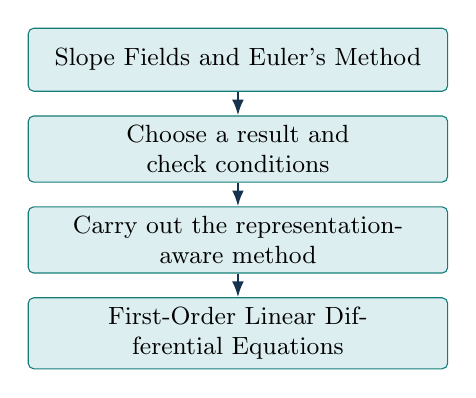
\begin{tikzpicture}[node distance=3mm, every node/.style={font=\small,align=center}, box/.style={draw=Teal,rounded corners=2pt,fill=Sky,minimum height=8mm,text width=0.42\textwidth}, arr/.style={-{Latex[length=2mm]},thick,draw=Ink}]
\node[box] (a) {Slope Fields and Euler's Method};
\node[box,below=of a] (b) {Choose a result and check conditions};
\node[box,below=of b] (c) {Carry out the representation-aware method};
\node[box,below=of c] (d) {First-Order Linear Differential Equations};
\draw[arr] (a)--(b); \draw[arr] (b)--(c); \draw[arr] (c)--(d);
\end{tikzpicture}
\end{center}
\end{minipage}

\section{Learning objectives}
\begin{enumerate}
\item Explain the central objects and hypotheses in 6.1 and 6.4.
\item Translate among algebraic, graphical, numerical, and verbal representations.
\item Select an appropriate formula or theorem before beginning symbolic work.
\item Carry out multi-step calculations while preserving domain, sign, orientation, and units.
\item Diagnose common errors by testing assumptions and checking the result independently.
\item Synthesize the chapter's methods into a reusable problem-solving workflow.
\end{enumerate}

\section{6.1 Slope Fields and Euler's Method}
\begin{longtable}{C N}\cornellcuehead
\cornellcuerow{What is the governing idea in 6.1?}{A slope field displays local derivatives, while Euler's method advances along tangent-line approximations.}
\cornellcuerow{Which result should be recalled?}{\formula{y_{n+1}=y_n+h f(x_n,y_n)}}
\cornellcuerow{How should a problem be organized?}{Plot representative slopes, choose step size $h$, update both coordinates, and compare numerical behavior with the field.}
\cornellcuerow{What should be checked before accepting an answer?}{Confirm the hypotheses and domain, preserve units and orientation when relevant, and substitute or differentiate back into the defining relation.}
\end{longtable}
\begin{warningbox}Using stale coordinates, changing step sign accidentally, or assuming smaller $h$ removes all error can mislead.\end{warningbox}
\begin{sectionsummarybox}A slope field displays local derivatives, while Euler's method advances along tangent-line approximations. The operational habit is to plot representative slopes, choose step size $h$, update both coordinates, and compare numerical behavior with the field.\end{sectionsummarybox}
\section{6.2 Growth and Decay}
\begin{longtable}{C N}\cornellcuehead
\cornellcuerow{What is the governing idea in 6.2?}{A quantity whose rate is proportional to itself follows an exponential law determined by an initial value.}
\cornellcuerow{Which result should be recalled?}{\formula{\frac{dy}{dt}=ky\quad\Longrightarrow\quad y=y_0e^{kt}}}
\cornellcuerow{How should a problem be organized?}{Identify the proportional-rate assumption, solve for $k$ from data, retain units of inverse time, and test long-term behavior.}
\cornellcuerow{What should be checked before accepting an answer?}{Confirm the hypotheses and domain, preserve units and orientation when relevant, and substitute or differentiate back into the defining relation.}
\end{longtable}
\begin{warningbox}The sign of $k$ controls growth versus decay; percent remaining and percent lost are not the same datum.\end{warningbox}
\begin{sectionsummarybox}A quantity whose rate is proportional to itself follows an exponential law determined by an initial value. The operational habit is to identify the proportional-rate assumption, solve for $k$ from data, retain units of inverse time, and test long-term behavior.\end{sectionsummarybox}
\section{6.3 Separation of Variables and the Logistic Equation}
\begin{longtable}{C N}\cornellcuehead
\cornellcuerow{What is the governing idea in 6.3?}{Separable equations isolate variables; logistic growth adds a carrying capacity that reduces the rate near saturation.}
\cornellcuerow{Which result should be recalled?}{\formula{\frac{dy}{dt}=ky\left(1-\frac{y}{K}\right)}}
\cornellcuerow{How should a problem be organized?}{Separate only where algebra permits, integrate both sides, apply the initial condition, and analyze equilibrium solutions separately.}
\cornellcuerow{What should be checked before accepting an answer?}{Confirm the hypotheses and domain, preserve units and orientation when relevant, and substitute or differentiate back into the defining relation.}
\end{longtable}
\begin{warningbox}Dividing by a factor involving $y$ may discard equilibrium solutions, and $K$ is not generally the initial value.\end{warningbox}
\begin{sectionsummarybox}Separable equations isolate variables; logistic growth adds a carrying capacity that reduces the rate near saturation. The operational habit is to separate only where algebra permits, integrate both sides, apply the initial condition, and analyze equilibrium solutions separately.\end{sectionsummarybox}
\section{6.4 First-Order Linear Differential Equations}
\begin{longtable}{C N}\cornellcuehead
\cornellcuerow{What is the governing idea in 6.4?}{An integrating factor converts $y'+P(x)y=Q(x)$ into the derivative of a product.}
\cornellcuerow{Which result should be recalled?}{\formula{\mu(x)=e^{\int P(x)dx},\qquad (\mu y)'=\mu Q}}
\cornellcuerow{How should a problem be organized?}{Put the equation in standard form, compute $\mu$, multiply every term, integrate, divide by $\mu$, and impose the initial condition.}
\cornellcuerow{What should be checked before accepting an answer?}{Confirm the hypotheses and domain, preserve units and orientation when relevant, and substitute or differentiate back into the defining relation.}
\end{longtable}
\begin{warningbox}Reading $P$ before normalizing the coefficient of $y'$ or failing to multiply the entire equation ruins the product structure.\end{warningbox}
\begin{sectionsummarybox}An integrating factor converts $y'+P(x)y=Q(x)$ into the derivative of a product. The operational habit is to put the equation in standard form, compute $\mu$, multiply every term, integrate, divide by $\mu$, and impose the initial condition.\end{sectionsummarybox}

\section{Definitions and theorem register}
\small
\begin{longtable}{@{}>{\RaggedRight\arraybackslash}p{0.24\textwidth}>{\RaggedRight\arraybackslash}p{0.40\textwidth}>{\RaggedRight\arraybackslash}p{0.29\textwidth}@{}}
\toprule
\textbf{Topic} & \textbf{Meaning and conditions} & \textbf{Canonical form}\\
\midrule\endhead
6.1 Slope Fields and Euler's Method & A slope field displays local derivatives, while Euler's method advances along tangent-line approximations. & \adjustbox{max width=\linewidth}{\(\displaystyle y_{n+1}=y_n+h f(x_n,y_n)\)} \\\addlinespace[2pt]
6.2 Growth and Decay & A quantity whose rate is proportional to itself follows an exponential law determined by an initial value. & \adjustbox{max width=\linewidth}{\(\displaystyle \frac{dy}{dt}=ky\quad\Longrightarrow\quad y=y_0e^{kt}\)} \\\addlinespace[2pt]
6.3 Separation of Variables and the Logistic Equation & Separable equations isolate variables; logistic growth adds a carrying capacity that reduces the rate near saturation. & \adjustbox{max width=\linewidth}{\(\displaystyle \frac{dy}{dt}=ky\left(1-\frac{y}{K}\right)\)} \\\addlinespace[2pt]
6.4 First-Order Linear Differential Equations & An integrating factor converts $y'+P(x)y=Q(x)$ into the derivative of a product. & \adjustbox{max width=\linewidth}{\(\displaystyle \mu(x)=e^{\int P(x)dx},\qquad (\mu y)'=\mu Q\)} \\\addlinespace[2pt]
\bottomrule
\end{longtable}
\normalsize

\section{Formula and method sheet}
\small
\begin{longtable}{@{}>{\RaggedRight\arraybackslash}p{0.08\textwidth}>{\RaggedRight\arraybackslash}p{0.48\textwidth}>{\RaggedRight\arraybackslash}p{0.37\textwidth}@{}}
\toprule
\textbf{Sec.} & \textbf{Method sequence} & \textbf{Stop-and-check trigger}\\
\midrule\endhead
6.1 & Plot representative slopes, choose step size $h$, update both coordinates, and compare numerical behavior with the field. & Using stale coordinates, changing step sign accidentally, or assuming smaller $h$ removes all error can mislead. \\\addlinespace[2pt]
6.2 & Identify the proportional-rate assumption, solve for $k$ from data, retain units of inverse time, and test long-term behavior. & The sign of $k$ controls growth versus decay; percent remaining and percent lost are not the same datum. \\\addlinespace[2pt]
6.3 & Separate only where algebra permits, integrate both sides, apply the initial condition, and analyze equilibrium solutions separately. & Dividing by a factor involving $y$ may discard equilibrium solutions, and $K$ is not generally the initial value. \\\addlinespace[2pt]
6.4 & Put the equation in standard form, compute $\mu$, multiply every term, integrate, divide by $\mu$, and impose the initial condition. & Reading $P$ before normalizing the coefficient of $y'$ or failing to multiply the entire equation ruins the product. \\\addlinespace[2pt]
\bottomrule
\end{longtable}
\normalsize

\section{Common errors and diagnostic checks}
\begin{warningbox}
\begin{itemize}
\item \textbf{6.1:} Using stale coordinates, changing step sign accidentally, or assuming smaller $h$ removes all error can mislead.
\item \textbf{6.2:} The sign of $k$ controls growth versus decay; percent remaining and percent lost are not the same datum.
\item \textbf{6.3:} Dividing by a factor involving $y$ may discard equilibrium solutions, and $K$ is not generally the initial value.
\item \textbf{6.4:} Reading $P$ before normalizing the coefficient of $y'$ or failing to multiply the entire equation ruins the product structure.
\end{itemize}
\end{warningbox}
\begin{checkbox}
Before accepting any result: state the relevant domain; check theorem hypotheses; estimate sign and scale; preserve units and orientation; and verify by substitution, differentiation, a limiting case, or a second representation.
\end{checkbox}

\section{Chapter synthesis}
Model rates of change with first-order differential equations and connect qualitative fields, numerical approximations, and analytic solution methods. The chapter begins with \textbf{Slope Fields and Euler's Method} and culminates in \textbf{First-Order Linear Differential Equations}. Across the sequence, the most reliable workflow is to identify the mathematical object, choose a representation, state the governing result with its hypotheses, compute without dropping restrictions, and audit the answer against the original definition. A differential equation solution is not just a formula: it must satisfy the rate law, the initial data, its domain, and the qualitative behavior predicted by the model.

\section{Self-test questions}
\begin{enumerate}
\item Explain the central distinction or object in 6.1, using both words and notation.
\item State the main formula or result from 6.2 and identify every hypothesis or restriction needed for its use.
\item Describe the problem-solving procedure for 6.3. What is the strongest independent check?
\item Compare the roles of Slope Fields and Euler's Method and First-Order Linear Differential Equations within this chapter.
\item Reconstruct the governing formula for 6.4 from its geometric or analytic meaning.
\item Choose one method in the chapter and explain how its output should be interpreted, including units or orientation when applicable.
\item Scenario: A student working on 6.1 produces a polished calculation but makes this error: Using stale coordinates, changing step sign accidentally, or assuming smaller $h$ removes all error can mislead. Diagnose the earliest invalid step and repair the workflow.
\item Scenario: A solution in 6.2 quotes the displayed formula without checking conditions. Which conditions must be checked, and what could fail if they are absent?
\item Construct a concept map linking a representation, a governing result, a computation, and a verification check from this chapter.
\item Design a two-part test for mastery: one conceptual prompt and one calculation. State what evidence would count as a complete answer.
\end{enumerate}

\Needspace{8\baselineskip}
\section{Answer key}
\small
\begin{enumerate}
\item A complete response identifies A slope field displays local derivatives, while Euler's method advances along tangent-line approximations. It should connect that meaning to \(y_{n+1}=y_n+h f(x_n,y_n)\) and state the relevant domain.
\item The organizing result is \(\frac{dy}{dt}=ky\quad\Longrightarrow\quad y=y_0e^{kt}\). The solver must check that the quantities are defined and that the assumptions named in 6.2 hold before applying it.
\item Use this sequence: Separate only where algebra permits, integrate both sides, apply the initial condition, and analyze equilibrium solutions separately. The strongest check is to return to the defining relation or differentiate/substitute the result, as appropriate.
\item Slope Fields and Euler's Method establishes a slope field displays local derivatives, while euler's method advances along tangent-line approximations. First-Order Linear Differential Equations extends the chapter to an integrating factor converts $y'+p(x)y=q(x)$ into the derivative of a product. The connection is the reuse of the same representations under a broader method.
\item The formula \(\mu(x)=e^{\int P(x)dx},\qquad (\mu y)'=\mu Q\) follows by translating the defining geometric or rate relationship into symbols; each factor records a distinct change or scale.
\item Interpretation must name what varies, with respect to what, and on which domain. A numerical value without units, sign, direction, or interval information is incomplete whenever those features are part of the modeled quantity.
\item The earliest fault is the unverified assumption described by this warning: Using stale coordinates, changing step sign accidentally, or assuming smaller $h$ removes all error can mislead. Restart by following this procedure: Plot representative slopes, choose step size $h$, update both coordinates, and compare numerical behavior with the field.
\item The formula \(\frac{dy}{dt}=ky\quad\Longrightarrow\quad y=y_0e^{kt}\) is conditional, not decorative. Check domain, differentiability or integrability as relevant, boundary or orientation requirements, and nonzero denominators before drawing a conclusion.
\item One valid map is: the representation in 6.1 identifies the object; the result in 6.2 supplies a rule; the method in 6.3 carries out the computation; the check in 6.4 tests the conclusion against its definition.
\item The conceptual prompt should require explanation of a definition and its hypotheses. The calculation should require method selection rather than direct substitution. Full evidence includes setup, justified transformations, a result, and an independent check.
\end{enumerate}
\normalsize

\section{Key-term recap}
\small
\begin{longtable}{@{}>{\RaggedRight\arraybackslash}p{0.29\textwidth}>{\RaggedRight\arraybackslash}p{0.64\textwidth}@{}}
\toprule
\textbf{Term} & \textbf{Working meaning}\\
\midrule\endhead
Slope Fields and Euler's Method & A slope field displays local derivatives, while Euler's method advances along tangent-line approximations. \\\addlinespace[2pt]
Growth and Decay & A quantity whose rate is proportional to itself follows an exponential law determined by an initial value. \\\addlinespace[2pt]
Separation of Variables and the Logistic Equation & Separable equations isolate variables; logistic growth adds a carrying capacity that reduces the rate near saturation. \\\addlinespace[2pt]
First-Order Linear Differential Equations & An integrating factor converts $y'+P(x)y=Q(x)$ into the derivative of a product. \\\addlinespace[2pt]
\bottomrule
\end{longtable}
\normalsize

\enlargethispage{4\baselineskip}
\begin{tcolorbox}[title=One-sentence takeaway,fonttitle=\bfseries,colback=Ink,colframe=Ink,coltext=white,coltitle=white,arc=2mm,boxrule=0pt]
\centering\bfseries A differential equation solution is not just a formula: it must satisfy the rate law, the initial data, its domain, and the qualitative behavior predicted by the model.
\end{tcolorbox}
\end{document}
